% !TEX encoding = UTF-8 Unicode
\level{1}{Resoconto delle varie attività di verifica - Fase SD} \label{app:esitiSD}
Anche durante questa terza fase, secondo quanto riportato dal \insdoc{Piano di Progetto v3.00}, sono previsti più momenti in cui viene attivato il processo di verifica. Si riportano in questa sezione tutti i risultati ottenuti durante questi momenti. Ove fosse necessario, sono state tratte anche delle conclusioni sui risultati ottenuti e su come essi possano essere migliorati.
	\level{2}{Verifica dei prodotti}
		\level{3}{Documenti}
			In questa sezione vengono riportati i risultati delle attività di verifica svolte sui documenti. Esse sono di due tipi:
			\begin{itemize}
				\item verifiche manuali;
				\item verifiche automatizzate.
			\end{itemize}
			\level{4}{Verifiche manuali}
				Le attività di verifica manuale della documentazione prodotta sono state svolte in base alla procedura riguardante la verifica dei 
				documenti che è descritta del documento \insdoc{Norme di Progetto v3.00}.\\
				La verifica manuale ha permesso di individuare soprattutto errori che riguardano le seguenti tipologie:
				\begin{itemize}
					\item descrizioni troppo sommarie laddove sono richieste descrizioni accurate e dettagliate;
					\item incongruenze tra parti diverse dello stesso documento o appartenenti a documenti diversi;
					\item errori nei concetti esposti.
				\end{itemize}
				Di seguito è presentato un riassunto della quantità di errori trovati (e successivamente risolti) utilizzando la verifica manuale durante l'intera \insphase{Fase SD}.
				\begin{table}[H]
					\centering
					\begin{tabu}{| l | c |}
						\hline
						Descrizioni sommarie	&	26\\ \hline
						Incongruenze	&	21\\ \hline
						Errori concettuali	&	12\\ \hline
					\end{tabu}
					\caption{Errori trovati tramite verifica manuale dei documenti durante la Fase SD}
				\end{table}
				Rispetto alla \insphase{Fase DB}, è stato riscontrato un aumento delle incongruenze tra i vari documenti. Ciò è dovuto al fatto che i documenti sono stati corretti in seguito alla prima revisione. Inoltre, in seguito ad alcuni incontri con il proponente, si è reso necessario apportare alcune modifiche alla progettazione.\\
				Durante la verifica manuale sono stati individuati nuovi termini da aggiungere al \insdoc{Glossario v3.00}. Di seguito è presentato un 
				riassunto della quantità di nuovi termini da aggiungere al \insdoc{Glossario v3.00} che sono stati individuati.
				\begin{table}[H]
					\centering
					\begin{tabu}{| l | c |}
						\hline
						Termini candidati ad essere aggiunti	&	12\\ \hline
						Termini aggiunti al \insdoc{Glossario v3.00}	& 10\\ \hline
					\end{tabu}
					\caption{Nuovi termini da inserire nel Glossario individuati tramite verifica manuale dei documenti durante la Fase SD}
				\end{table}
				È stata infine verificata la correttezza dei diagrammi UML utilizzati all'interno dei vari documenti, sempre seguendo le procedure contenute nel documento \insdoc{Norme di Progetto v3.00}. Per quanto riguarda i diagrammi delle componenti non sono stati riscontrati grossi problemi. Sì è rivelata più critica la stesura dei diagrammi di attività inerenti le modalità di interezione tra le varie componenti.
				
			\level{4}{Verifiche automatizzate}
			Le attività di verifica automatizzate, oltre a rispettare le procedure descritte all'interno delle \insdoc{Norme di Progetto v3.00}, fanno uso degli strumenti automatici previsti all'interno dello stesso documento. Questi hanno permesso di individuare numerosi errori che riguardano le seguenti tipologie:
			\begin{itemize}
				\item ortografia errata;
				\item utilizzo errato dei comandi \LaTeX{} previsti dalle \insdoc{Norme di Progetto v3.00};
				\item norme tipografiche non rispettate.
			\end{itemize}
			Di seguito è presentato un riassunto della quantità di errori trovati (e successivamente risolti) utilizzando la verifica automatica.
			\begin{table}[H]
					\centering
					\begin{tabu}{| l | c |}
						\hline
						Errori ortografici	&145	\\ \hline
						Utilizzo errato \LaTeX{}	&3	\\ \hline
						Errori riguardanti norme tipografiche	&11	\\ \hline
					\end{tabu}
					\caption{Errori trovati tramite verifica automatica dei documenti durante la Fase SD}
				\end{table}
				Come si può notare, gli errori di utilizzo errato dei comandi \LaTeX{} e gli errori relativi le norme tipografiche sono diminuiti rispetto alla \insphase{Fase DB}. Ciò è probabilmente dovuto ad una maggiore familiarità del team con le \insdoc{Norme di Progetto v3.00}.\\
				Di seguito riportiamo gli indici ottenuti dal calcolo dell'indice di leggibilità sui documenti completi.
				\begin{table}[H]
					\centering
					\begin{tabu}{| l | c | c |}
							\hline
							Documenti 							& Gulpease	& Esito		\\ \hline \hline
							
							Piano di progetto v3.00				& -- 		& Superato  \\ \hline
							Norme di Progetto v3.00 			& --		& Superato  \\ \hline
							Piano di Qualifica v3.00 			& --		& Superato  \\ \hline
							Specifica Tecnica v1.00 			& --		& Superato  \\ \hline
							Glossario v3.00					 	& -- 		& Superato  \\ \hline
						\end{tabu}
					\caption{Esiti del calcolo dell'indice di leggibilità effettuato tramite strumenti automatici durante la Fase SD}
				\end{table}
	\level{2}{Verifica dei processi}
		\level{3}{Processo di documentazione}
			\level{4}{Livello CMM}
			Questa fase è cominciata con un livello CMM pari a 2. In seguito alla riorganizzazione delle \insdoc{Norme di Progetto v3.00} e del \insdoc{Piano di Qualifica v3.00}, e grazie ad una maggiore esperienza dei membri del team, i processi e la loro organizzazione sono notevolmente migliorati. Ciò ha permesso di raggiungere il terzo livello CMM. In questa fase abbiamo, inoltre, iniziato a misurare la qualità dei processi ampliando le metriche utilizzate. Il nostro obiettivo è raggiungere via via un maggiore dettaglio nella misurazione della qualità dei processi, in modo da avere un migliore controllo sulla qualità.
			\level{4}{Schedule Variance}
			La maggior parte delle attività pianificate nel \insdoc{Piano di Progetto v3.00} sono state svolte rispettando le scadenze. La parte in cui il gruppo ha riscontrato maggiori problemi è stata la \insdoc{Specifica Tecnica v1.00}. In particolare ci sono stati ritardi nella progettazione delle componenti. Ciò è dovuto principalmente all'inesperienza del gruppo unita alla difficoltà di progettazione di un buon framework.\\
			Riportiamo di seguito i valori ottenenuti calcolando la Schedule Variance sui tempi di stesura di ogni documento:
			\begin{table}[H]
					\centering
					\begin{tabu}{| l | c | c |}
							\hline
							Documenti 							& Schedule Variance	& Esito		\\ \hline \hline
							
							Piano di progetto v3.00				& 0\% 		& Ottimale  \\ \hline
							Norme di Progetto v3.00 			& 4\%		& Ottimale  \\ \hline
							Piano di Qualifica v3.00 			& 1\%		& Ottimale  \\ \hline
							Specifica Tecnica v1.00 			& -21\%		& Non Accettabile  \\ \hline
							Glossario v3.00					 	& 13\% 		& Ottimale  \\ \hline
							Totale processo di documentazione & -3\% & Accettabile \\ \hline
						\end{tabu}
					\caption{Esiti del calcolo della Schedule Variance durante la Fase SD}
				\end{table}
			\level{4}{Budget Variance}
			Le risorse necessarie all'incremento dei documenti \insdoc{Norme di Progetto v3.00} e \insdoc{Glossario v3.00} si sono rivelate leggermente inferiori rispetto a quelle preventivate. Al contrario, le risorse impiegate per la stesura della \insdoc{Specifica Tecnica v1.00} sono state maggiori rispetto al pianificato. In particolare, la Bugdet Variance specifica di quest'ultimo documento ha un valore non accettabile. Nonostante ciò, nel complesso il bilancio è positivo.\\
			Riportiamo di seguito i valori ottenenuti calcolando la Budget Variance sulle risorse utilizzate per la stesura di ogni documento:
			\begin{table}[H]
					\centering
					\begin{tabu}{| l | c | c |}
							\hline
							Documenti 							& Budget Variance	& Esito		\\ \hline \hline
							
							Piano di progetto v3.00				& 0\% 		& Ottimale  \\ \hline
							Norme di Progetto v3.00 			& 13\%		& Ottimale  \\ \hline
							Piano di Qualifica v3.00 			& 1\%		& Ottimale  \\ \hline
							Specifica Tecnica v1.00 			& -15\%		& Non accettabile  \\ \hline
							Glossario v3.00					 	& 5\% 		& Ottimale  \\ \hline
							Totale processo di documentazione & 14\% & Ottimale \\ \hline
						\end{tabu}
					\caption{Esiti del calcolo della Budget Variance durante la Fase SD}
				\end{table}

			\level{4}{Produttività}
			Utilizzando la formula descritta all'interno del presente documento (sezione \nameref{sec:metriche}) è stata calcolata la produttività del processo di documentazione. Questo indice è stato calcolato durante tutti i momenti di verifica previsti dal \insdoc{Piano di Progetto v3.00} per	la \insphase{Fase SD}, e ciò è stato fatto per ogni documento che è stato redatto nel periodo antecedente la verifica. Ogni documento è stato sottoposto al processo di verifica al più cinque volte. Il calcolo fatto di volta in volta sullo stesso documento tiene conto solo delle nuove sezioni introdotte in esso.\\
				Segue un riassunto di quanto è stato fatto.
				\begin{table}[H]
					\centering
					\begin{tabu}{| l | c | c | c | c | c |}
						\hline
							&1	&2	&3	&4	&5	\\ \hline
						Norme di Progetto	& 186 &	&	&	& \\ \hline
						Specifica Tecnica &	209 & 154 & 46	&	128 & 189 \\ \hline
						Piano di Progetto	& 163 &	&	&	& \\ \hline
						Piano di Qualifica	& 201	&	&	&	&\\ \hline
						Glossario & 152 & 74 & & &\\ \hline
					\end{tabu}
					\caption{Produttività delle varie attività del processo di documentazione durante la fase SD}
				\end{table}
				Di seguito vengono riportati in un grafico i valori della produttività del processo di documentazione rilevati nei vari periodi della \insphase{Fase SD} nei quali è stato applicato il processo di verifica. Il grafico fa riferimento alla tabella precedente.\\
				\begin{figure}[H]
					\centering
					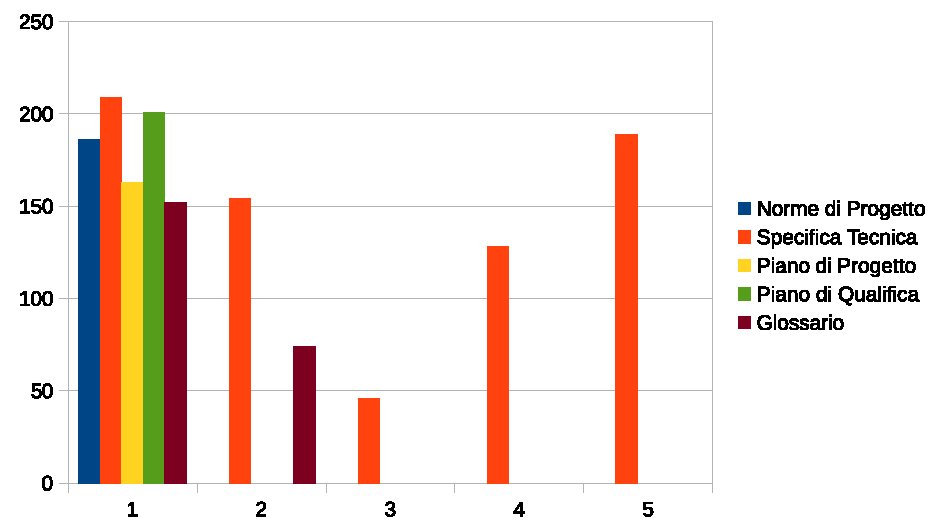
\includegraphics[width=12cm]{PianoDiQualifica/Pics/ProduttivitaDocumentazioneFaseSD.pdf}
					\caption{Produttività del processo di documentazione durante la Fase SD}
				\end{figure}
				Dal grafico si può notare che i documenti che hanno subito un incremento rispetto alle fasi precedenti mantengono una produttività discretamente elevata. L'unica eccezione è costituita dal \insdoc{Glossario v3.00}, la cui produttività cala dopo il secondo incremento. Ciò è dovuto al fatto che i termini da inserire in tale documento sono stati individuati quasi tutti durante il primo incremento. L'abbassamento della produttività è dunque imputabile ad un ridotto numero di parole nuove durante il secondo incremento.\\
				Va fatto un discorso a parte per la \insdoc{Specifica Tecnica v1.00}. La produttività di tale documento subisce un brusco calo durante l'attività di progettazione delle componenti. Questa attività è stata infatti rallentata a causa delle opinioni discordi dei progettisti su quale fosse la soluzione progettuale migliore.
			
		\level{3}{Processo di verifica}
			\level{4}{Livello CMM}
			In questa fase, durante il processo di verifica abbiamo cominciato ad utilizzare un maggior numero di metriche per cercare di misurare la qualità dei processi verificati. Il processo di verifica ha dunque acquisito un valore aggiunto rispetto alle fasi precedenti. Inoltre, in seguito all'aggiunta di norme inerenti la gestione del processo di verifica e in seguito alla revisione delle strategie di verifica, si può dire che questo processo abbia raggiunto il terzo livello CMM. 
			\level{4}{Schedule Variance}
			Il processo di verifica è stato sempre svolto rispettando le scadenze temporali previste nel \insdoc{Piano di Progetto v3.00}. I valori della Schedule Variance calcolati per questo processo risultano quindi ottimi.\\
			Riportiamo di seguito il valore ottenenuto:
			\begin{table}[H]
					\centering
					\begin{tabu}{| l | c | c |}
							\hline
							Processi 							& Schedule Variance	& Esito		\\ \hline \hline
							Processo di verifica & 0\% & Ottimale \\ \hline
						\end{tabu}
					\caption{Esiti del calcolo della Schedule Variance durante la Fase SD}
				\end{table}	

			\level{4}{Budget Variance}
			Le risorse utilizzate nel processo di verifica sono maggiori rispetto a quelle preventivate. Il valore della Budget Variance per questo proceso risulta non accettabile.\\ 
			Riportiamo di seguito il valore ottenenuto:
			\begin{table}[H]
					\centering
					\begin{tabu}{| l | c | c |}
							\hline
							Processi 							& Budget Variance	& Esito		\\ \hline \hline
							Processo di verifica & -11\% & Non accettabile \\ \hline
						\end{tabu}
					\caption{Esiti del calcolo della Budget Variance durante la Fase SD}
				\end{table}	
							
			\level{4}{Produttività}
			Utilizzando la formula descritta all'interno del presente documento (sezione \nameref{sec:metriche}) è stata calcolata la produttività del processo di verifica. Tale indice è stato calcolato in seguito a tutti i momenti di verifica previsti dal \insdoc{Piano di Progetto v3.00} per la \insphase{Fase SD}. Di seguito vengono riportati i valori calcolati e una loro rappresentazione grafica.
			\begin{table}[H]
					\centering
						\begin{tabu}{| c | c |}
							\hline
							Data verifica &Produttività\\ \hline \hline
							07/03 &1 \\ \hline
							08-09/03 & 5 \\ \hline
							14-15/03 & 3 \\ \hline
							18-21/03 & 3 \\ \hline
							20-21/03 & 14 \\ \hline
							26-27/03 & 12 \\ \hline
							28-31/03 & 11 \\ \hline
							31/03-01/04 & 7  \\ \hline
							01-02/04 & 1 \\ \hline
							02/04 & 4 \\ \hline							
						\end{tabu}
					\caption{Produttività del processo di verifica durante la fase SD}
				\end{table}
				\begin{figure}[H]
					\centering
					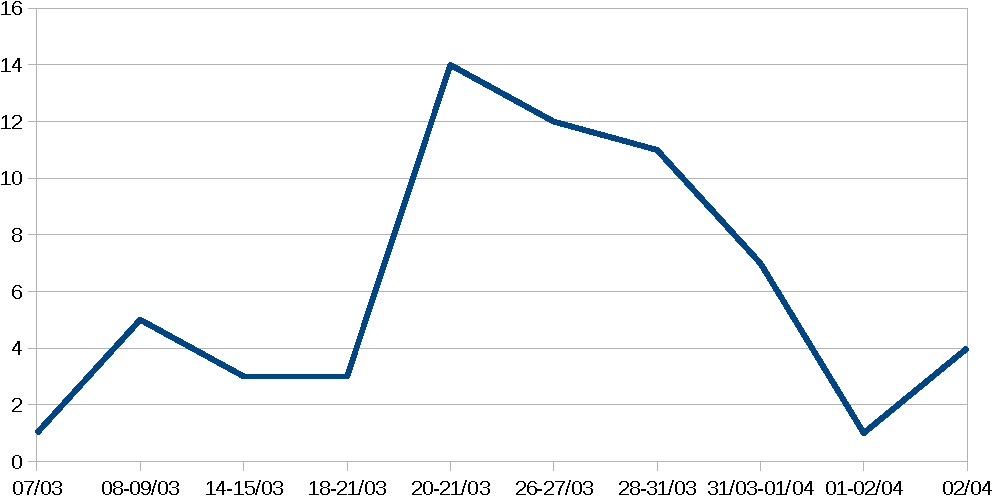
\includegraphics[width=12cm]{PianoDiQualifica/Pics/ProduttivitaVerificaFaseSD.pdf}
					\caption{Produttività del processo di verifica durante la Fase SD}
				\end{figure}
				Si può notare che la produttività delle attività di verifica è in media più bassa rispetto alla \insphase{Fase DB}. Ciò è dovuto ad una notevole diminuzione delle anomalie all'interno dei documenti a cui sono stati apportati incrementi. Sono presenti dei picchi in corrispondenza delle verifiche al documento \insdoc{Specifica Tecnica v1.00}. Ciò è probabilmente dovuto al fatto che questa è la prima esperienza di progettazione software per tutti i membri del team, dunque il numero di errori riscontrati durante l'attività di verifica è elevato.

			\level{4}{Efficacia di una revisione}
			Utilizzando la formula descritta all'interno del presente documento (sezione \nameref{sec:metriche}) è stata calcolata l'efficacia delle varie revisioni che sono state fatte durante la \insphase{Fase SD}. Di seguito vengono riportati i valori calcolati e una loro rappresentazione grafica.
				\begin{table}[H]
					\centering
						\begin{tabu}{| c | c |}
							\hline
							Data verifica &Efficacia\\ \hline \hline
							07/03 & -- \\ \hline
							08-09/03 & -- \\ \hline
							14-15/03 & -- \\ \hline
							18-21/03 & -- \\ \hline
							20-21/03 & -- \\ \hline
							26-27/03 & -- \\ \hline
							28-31/03 & -- \\ \hline
							31/03-01/04 & --  \\ \hline
							01-02/04 & -- \\ \hline
							02/04 & -- \\ \hline							
						\end{tabu}
					\caption{Produttività del processo di verifica durante la fase SD}
				\end{table}
				GRAFICO\\ \\
				%\begin{figure}[H]
				%	\centering
				%	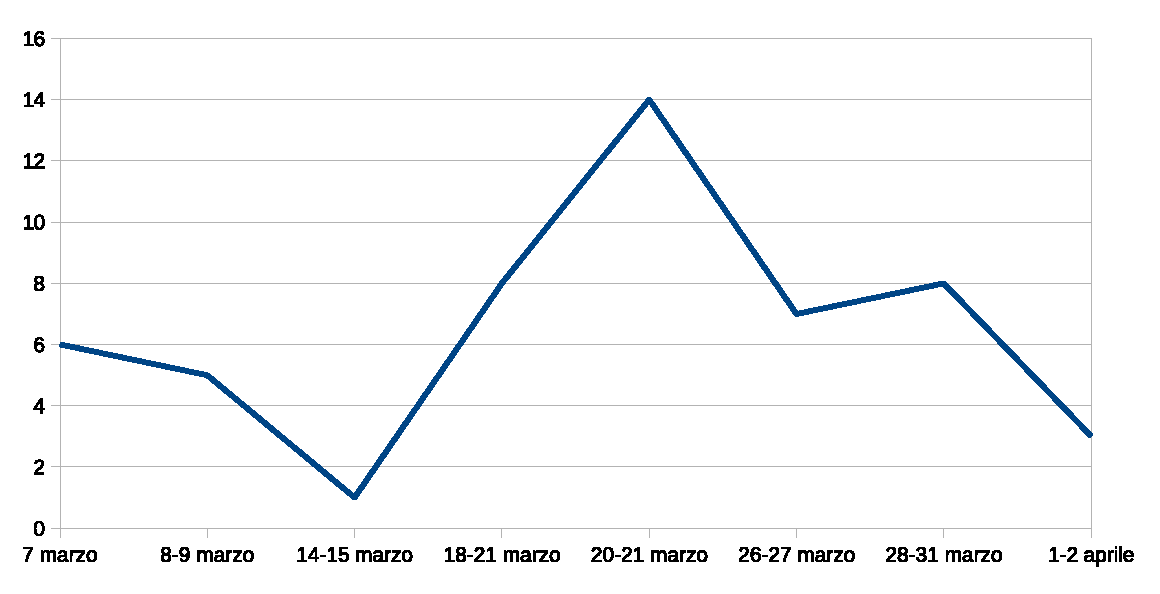
\includegraphics[width=12cm]{PianoDiQualifica/Pics/EfficaciaRevisioniFaseSD.pdf}
				%	\caption{Efficacia delle revisioni durante la Fase SD}
				%\end{figure}
				L'andamento dell'efficacia delle attività di verifica rispecchia l'andamento della produttività:
				\begin{itemize}
					\item in generale si ha un'efficienza bassa, dovuta ad un ridotto numero di errori rilevati nei documenti ai quali è stato apportato un incremento;
					\item durante le attività di verifica del documento \insdoc{Specifica Tecnica v1.00} l'efficienza aumenta, fino a raggiungere un picco in corrispondenza della verifica della progettazione delle componenti.
				\end{itemize}
		\level{3}{PDCA}
		In questa sezione viene riportato il grafico PDCA della \insphase{Fase SD}. In ascissa è rappresentato il tempo, in ordinata le attività.
		GRAFICO\\ \\
		%\begin{figure}[H]
		%		\centering
		%		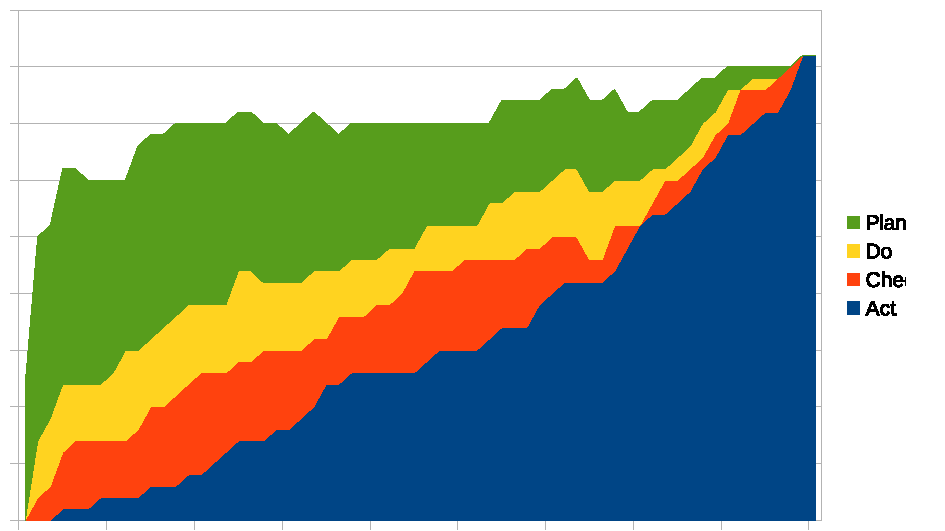
\includegraphics[width=0.6\textwidth]{PianoDiQualifica/Pics/GraficoPDCAFaseSD.pdf}
		%		\caption{PDCA Fase SB}
		%\end{figure}
